\chapter{Theoretische Grundlagen}
In this section the theoretical foundation of this thesis will be laid to understand the problem and the components used to solve it. First the dataset KIT-Motion Dataset combines both the motion themselves as xml-Data in the mmm-format, and to each motion a textual annotation has been assigned. Thus making it semantically rich and allowing natural language processing to be used to solve the problem.
\section{Human activity recognition}\label{sec:HAR}
In the fields of medicine, surveillance and sports human activity recognition plays a great role. Applications of HAR are intra-disciplined and range from surveillance of the elderly, high-performance sport and quantifying the calorie consumption based on the performed human activities. To implement this, it might be very helpful to use sensors to know the relative position of a body part, its speed and it acceleration, which is also the base for this thesis. This approach is very promising, due to the prevalent nature of wearables capable of capturing these information. Here, some of the methods used in practice are outlined and the difficulties encountered by researchers to have a picture of the state of the art in HAR and how it was achieved.\newline
First, the shape-based methods have received a lot of attention since the 2000s, where the human body is described in 2D space as rectangular patches and as volumetric shapes in 3D spaces. In other words, the human body is reduced to a silhouette consisting of limbs jointly connected to each other. This approach is relevant in classifying human motions captured in videos\cite{vrigkas2015review}. This makes classifying motion captured on videos feasible and proves that temporal-spacial input for classifying motions is relevant for this task. However, the identification of the body parts contribute the most to the task of activity recognition remain challenging and requiring the use of hierarchical composition model such as in \cite{lillo2014discriminative}. Lillo et al. showed that hierarchical compositional models reach a high level of precision in determining, which actions are performed by a person and the relevant part for it. In addition to that, their model could determine, if a person is performing multiple tasks at the same time, i.g. walking while having a phone call, and could discriminate between actions that can't be performed at the same time. In other words, their model builds a discriminative dictionary of body pose primitives, which are combined to compose atomic actions at a low level. Consequentially, these atomic actions are combined to compose complex activities at the top level\cite{lillo2014discriminative}.\newline
Another approach is using the multimodal methods, which were the focus of recent studies and attempts to tackle this problem. Here, events are seen as ensemble of of values of some descriptors, i.e. the position of the arm ans its velocity, in a moment. Thus providing the model with more useful information. However, the collected information should be be somehow fused together in a meaningful way, and making feature fusion a necessary tool to achieve this. One can differentiate between two extreme strategies: early and late fusion, though a hybrid approaches exists, such as slow fusion and single frame as illustrated in fig \ref{fig:feature_fusion} and explained in more details in \ref{subsec:feature-fusion}. In the context of classifying human activities by using information about the positions of the joints feature fusion could make the trained models very robust against occlusion and noise and could improve the recognition performance\cite{vrigkas2015review}.
\subsection{Feature Fusion}\label{subsec:feature-fusion}
The need to use feature fusion for the task of human activity recognition is due to the fact, that this can be achieved by using an multitude of input, i.g visual or auditory. In this thesis only information about the joints and the position of the pelvis is taken into account. However, each joint is positioned in an axis, thus making it useful to use feature fusion in this context. Karpathy et al. investigated fusing information across temporal domain using multiple methods listed in fig \ref{fig:feature_fusion}. In principle, the fusion can be used in the early stages in a CNN by modifying the first convolutional layer in the network and extending them in time. Another approach is to delay the fusion and replace the first layer by two temporally separate single-frame networks. Later can the fusing of the output of the two single-frame networks take part\cite{karpathy2014large}.\newline
% TODO Continue the explanation of feature fusion by using the paper {karpathy2014large}
\begin{description}
	\item[Single frame] TOBEFILLED
	\item[Slow fusion] TOBEFILLED
	\item[Late fusion] TOBEFILLED
	\item[Early fusion] TOBEFILLED
\end{description}
\begin{figure}
	\centering
	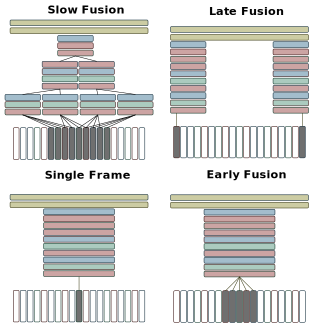
\includegraphics[width=\textwidth]{img/feature_fusion.pdf}
	\caption{Representation of fusion of information as shown in \cite{karpathy2014large}}
	\label{fig:feature_fusion}
\end{figure}
\subsection{Inherent Problems with HAR}\label{subsec:probHAR}
\section{Natural Language Processing}
Natural language processing began 1950 as the intersection of artificial intelligence and linguistics. At first it was very distinguishable from test information retrieval, where researchers employed highly scalable statistical techniques to index and search large volumes of text in an efficient manner\cite{nadkarni2011natural}. Nowadays the two domains converged to create the new NLP field of study, where researchers are required to borrow from other fields to create new methods of analysing and interpreting information in a textual or spoken from.\newline
With Chomskey's 1956 theoretical analysis of language grammars an estimate the complexity of the problems in NLP was provided, and influenced the creation of the Backus-Naur Form. This notation specified context-free grammars and is the base of programming language representations. In addition to that Chomskey found more restrictive Grammars, regular grammars, which are used to specify text-search patterns\cite{nadkarni2011natural}. These constructs were first the base of the first logical programming language Prolog, which syntax was conceived to suite writing grammars.\newline
These approaches in the early days relied heavily on symbolic and hand-crafted rules, and didn't contribute to the semantic analysis, i.e. extracting the meaning, but were used to syntactically analyse text and to check the syntactic consistency of programs. Nevertheless these formal grammars can specify the relationship between text units, and the can be extended semantically by expanding sub-categorization and adding more rules and constrains. However this leads to an explosion of the number of rules and leading to an unmanageable and unpredictable interactions\cite{nadkarni2011natural}.\newline
In the 1980s, NLP pivoted drastically into a statistical approach outlined by Klein\cite{kleincs}, where using simple and robust approximations ans outlined above was replaced by deep analysis with leaning machines, e.g. Transformers..., which used probabilities and were trained by large and annotated corpora. More so, the evaluation of the trained learning machines was more diligent and precise\cite{nadkarni2011natural}. This birthed the model statistical NLP, where the hand-crafted rules were replaced by broader rules having a probabilities determined through the trained machine learning\cite{kleincs}. In the practical part of this thesis some low-level NLP tasks will be used to extract and determine the class of each motion with its annotation. Tokenizers are an example to a low-level NLP task, where the individual tokens, i.e. words and punctuations, are identified. To achieve this a lexer is used to divide the text into lists of subtexts, that are then used in the next steps of the syntactical and semantic analysis of the text.\newline
\subsection{Word taggers}\label{subsec:wordtaggers}
A central task in this thesis is the syntactic analysis of texts ans speech and assign to each identified token a tag, i.e. the position and the role in the sentence\cite{nadkarni2011natural}. To this end Matthew Honnibal implemented a part of speech tagger to tag tokens in a sentence, where he used an averaged perceptron. Here a table of data is provided, but the last column, i.e. the position of each token in the sentence. \cite{honnibal_2013} 
% TODO Complete the NLP section with base https://explosion.ai/blog/part-of-speech-pos-tagger-in-python
\subsection{Stemmer}\label{subsec:stemmer}
\section{Classification of Time Series}
Time series are of ubiquitous nature and occur in nature in a multitude of ways, such as weather patterns and physiological signals, and also in human activities, such as financial recording. This makes their classification a cross domain task, with a very string baseline. Understanding this problem and solving it may influence the domain of machine learning in a significant way\cite{wang2017time}. Recently, it has been demonstrated that data-driven approaches is pivotal for data mining tasks by using deep learning methods and algorithms. A typically used learning machine for this is the ANN(Artificial Neural Network), which has proven to be capable of matching complicated functions leading to its popularity. A very special kind of ANNs is the CNN(Convolutional Neural Network), which has been primarily used for the task of image classification for its ability of extracting spatial features. However, the use of CNNs for the task of classification of time series remain very limited and challenging. On the other hand, RNN(Recurrent Neural Networks) are suitable for this task as it effectively uses the temporal nature of time series.\cite{yang2019time}
\subsection{Deep neural networks}
In the paper \cite{yang2019time} a standard baseline is established to exploit deep neural networks for end-to-end time series classification without the need of preprocessing and feature engineering. The authors evaluated a suite of learning machines:
\begin{itemize}
	\item MLP(Multilayer Perception).
	\item FCN(Fully convolutional Network).
	\item ResNet(Residual Network).
\end{itemize}
The conclusion of this comparative study is that ResNets and FCNs in a pure end-to-end training achieved better performance than COTE(Collective of Transformation-Based Ensembles)\cite{2015TSClassificationCOTE}. In addition to that, the use of global average pooling in the convolution layers in the models in the study enabled the exploitation of CAM(Class Activation Map). Thus finding our the contributing regions in the time series to the specific class\cite{wang2017time}. In the fig\ref{fig:wang2017time} the used architectures are illustrated.
\begin{figure}
	\centering
	\begin{subfigure}[b]{0.25\textwidth}
		\centering
		\includegraphics[width=\textwidth]{img/mlp.pdf}
		\caption{MLP}
		\label{fig:wang2017timemlp}
	\end{subfigure}
	\hfill
	\begin{subfigure}[b]{0.25\textwidth}
		\centering
		\includegraphics[width=\textwidth]{img/fcn.pdf}
		\caption{FCN}
		\label{fig:wang2017timefcn}
	\end{subfigure}
	\hfill
	\begin{subfigure}[b]{0.3\textwidth}
		\centering
		\includegraphics[width=\textwidth]{img/resnet.pdf}
		\caption{ResNet}
		\label{fig:wang2017timeresnet}
	\end{subfigure}
	\caption{The network structure of three tested neural networks. Dash line indicates the operation of dropout\cite{wang2017time}.}
	\label{fig:wang2017time}
\end{figure}
% TODO continue with wang2017time
\subsection{RNNs und LSTMs}
% \section{Decoder-Encoders}
% \section{Transformers}
% \section{Multi-head self-attention}
% \section{positional encoder}
% \section{BERT}
% \section{Embedding Models}
